

\red{1) on explique la discretisation}\newline
\red{2) on explique que sauf pour le first step, on a }
$$f(U)=A*U$$ et on \red{défini la matrice A}. Cela because en gros

For any index $t$,
\begin{align*}
f(U_i ) &= \frac{\nu}{r_i}\dfrac{(U_{i+1}-U_{i-1})}{h_x}+\nu\dfrac{U_{i+1}-2U_{i}+U_{i-1}}{h_{x}*h_{x}} -\frac{\nu}{r_{i}^2}U_{i}\\
&= \frac{\nu}{h_x}\Big( \frac{1}{h_x} - \frac{1}{r_i}\Big)U_{i-1} 
 -\nu\Big( \frac{2}{h_{x}^2} + \frac{1}{r_{i}^{2}}\Big)U_{i}
+ \frac{\nu}{h_x}\Big( \frac{1}{h_x} + \frac{1}{r_i}\Big)U_{i+1}\\
\end{align*} 

So we can now write the Crank-Nicolson method as
\begin{align*}
U^{t+1} &= U^{t} + 0.5*h_{t}\Big(f(U^{t}) + f(U^{t+1})\Big)\\
  &= U^{t} + 0.5*h_{t}\Big(A*U^{t} + A*U^{t+1}\Big)\\
\end{align*}

Therefore,
$$\Big(Id -0.5*h_{t}*A\big)U^{t+1} = (Id + 0.5*h_{t}*A)U^{t}$$
This is a linear system that can easily be solved for $U^{t+1}$.\newline

\red{TODO: jacobien est minus donc c'est stiff, analyser la condition CFL pour voir si les pas choisis ont du sens etc}







\begin{figure}[!h]
\centering
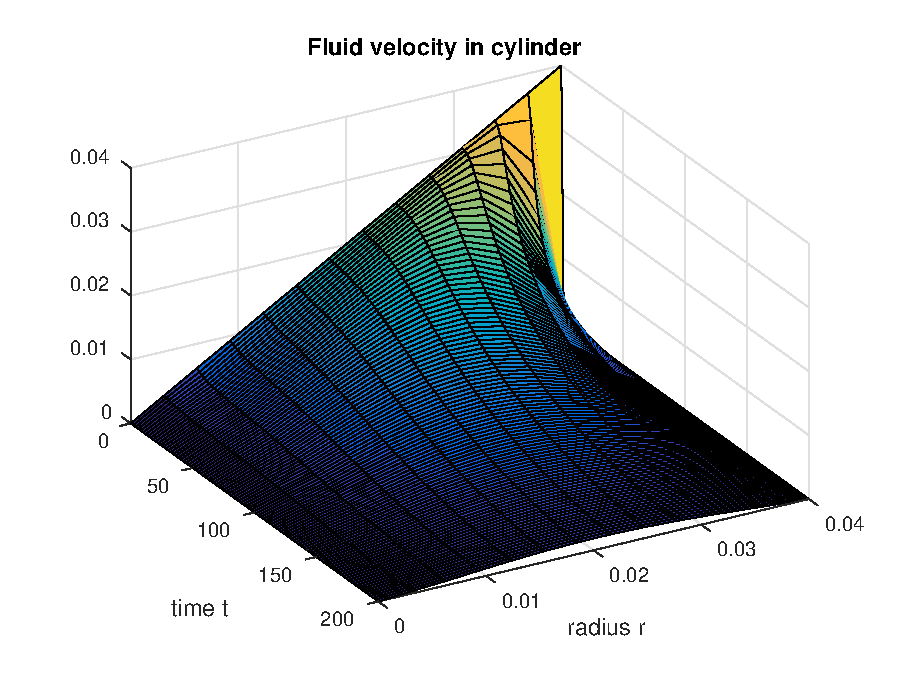
\includegraphics[width = 0.7\textwidth]{./dim1.eps}
\caption{Solution for one dimension}
\label{fig:dim1sol}
\end{figure}
\FloatBarrier
